\section{文字與字型 Rendering}

\subsection{FreeGLUT 字型}
\label{sec:glut-font}

文字物件保存左上角位置、UTF-8 字串與字型樣式。FreeGLUT 內建兩類字型：Bitmap Font 以 \lstinline|glRasterPos2f()| 指定位置後呼叫 \lstinline|glutBitmapCharacter()|，由於 raster position 對應字元基線附近，程式依各字型的高度與 origin 偏移，將「行頂端」換算為基線位置；Stroke Font 以線段描述字元，座標 Y 軸向上，繪製前先平移到基線，再以 \lstinline|glScalef(s, -s, 1)| 縮放並翻轉 Y 軸以配合 Canvas。兩者都逐 byte 繪製，只涵蓋 ASCII，無法顯示中文。

\subsection{UTF-8 解碼}
\label{sec:utf8-decode}

為了支援中文，字串在繪製與編輯前都先由 UTF-8 解碼為 Unicode code point，之後的游標移動、字形查找都以 code point 為單位。不合法的 byte 序列一律轉為替代字元 U+FFFD，且只略過 1 byte，讓後續合法的字元仍能正確解碼。

\subsection{文字輸入}
\label{sec:text-input}

UTF-8 的一個字元可能佔 1 到 4 bytes，例如「你」編碼為 \texttt{E4 BD A0} 三個 bytes。若直接在 \lstinline|std::string| 上以 byte 移動游標或刪除，游標可能停在字元中間，如圖~\ref{fig:utf8-caret} 下排的紅線，此時 Backspace 會留下無法解碼的殘缺 bytes。因此輸入框以 code point 陣列作為編輯資料，游標只會停在圖中上排的字元邊界，Backspace 與 Delete 一次刪除一個完整字元；內容改變後才重新編碼為 UTF-8 字串供外部使用。

\begin{figure}[htbp]
    \centering
    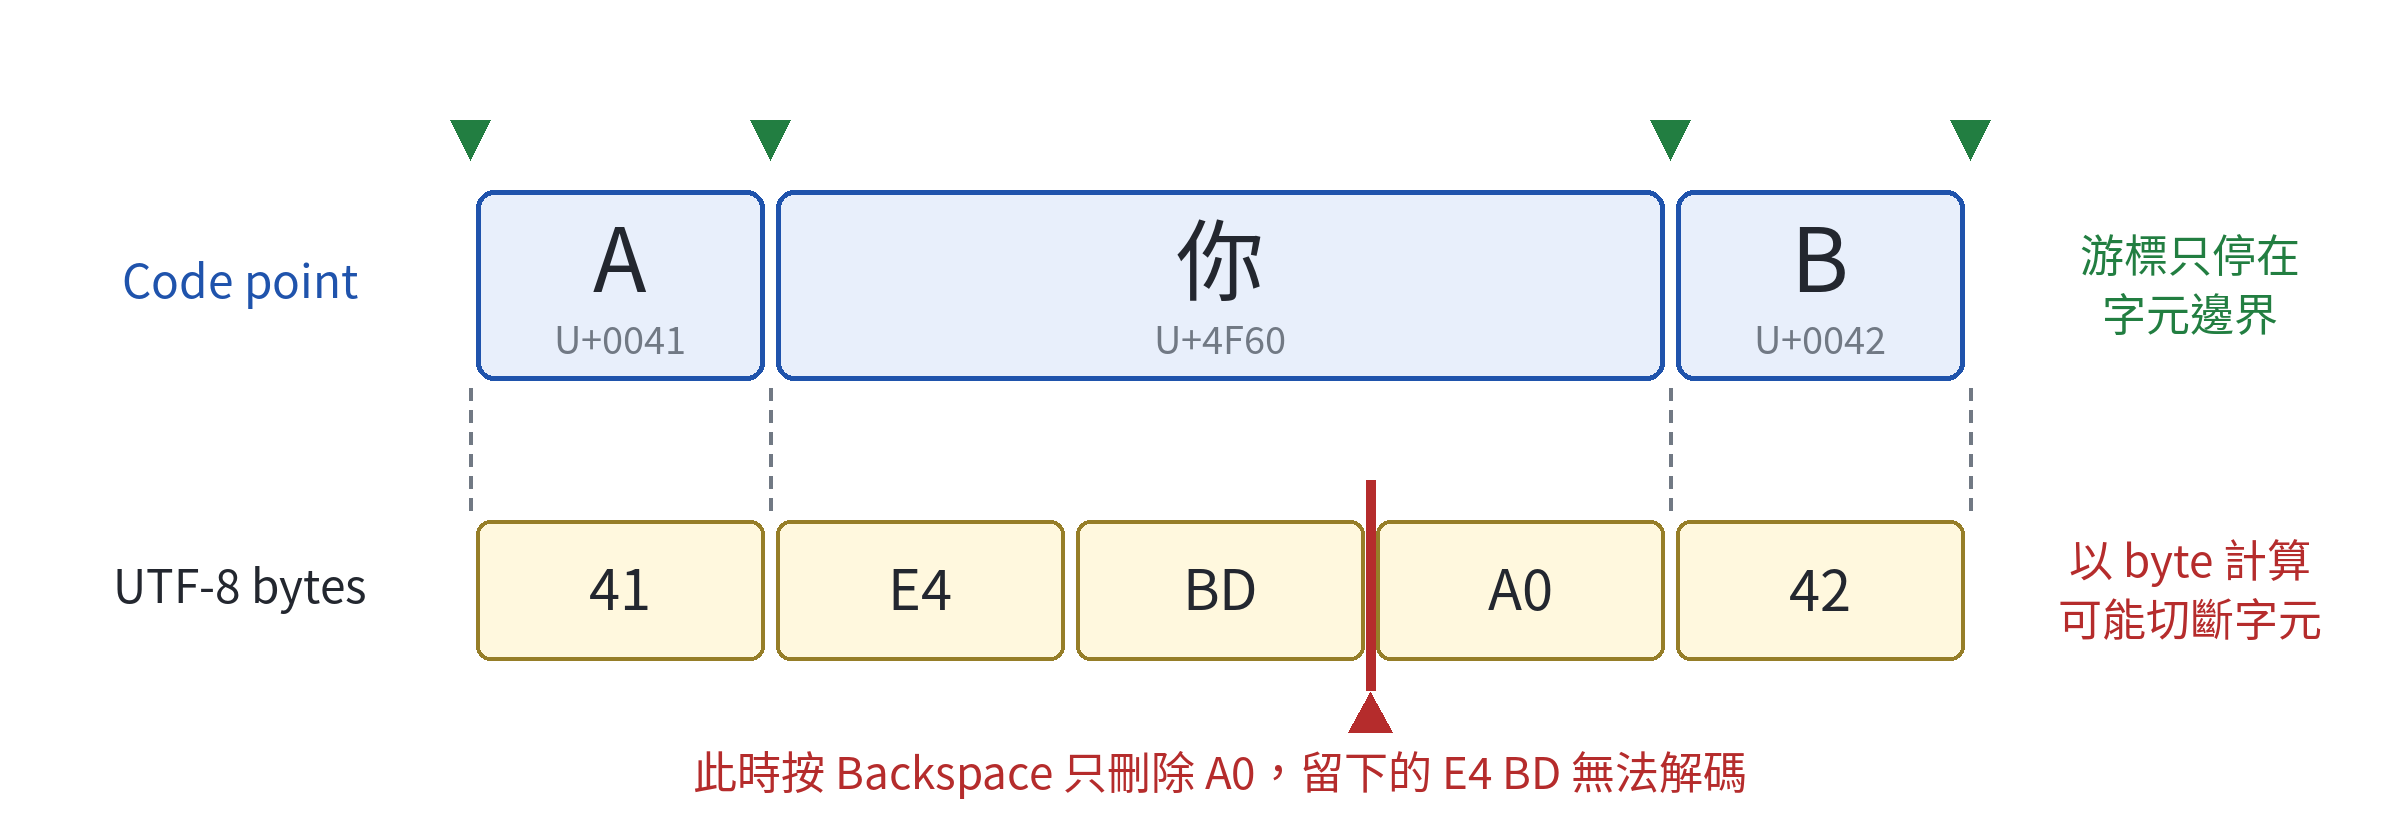
\includegraphics[width=.8\textwidth]{docs/figures/ch05_utf8-caret.png}
    \caption{同一字串的 code point 與 UTF-8 bytes 對照。以 byte 為單位移動游標可能切斷多 byte 字元，因此輸入框以 code point 為單位編輯}
    \label{fig:utf8-caret}
\end{figure}

FreeGLUT 的鍵盤 callback 每次只提供一個 byte，無法接收輸入法組字的結果。為此輸入框提供 Unicode 輸入模式：輸入反引號 \texttt{`} 後接 4 位十六進位數字，即可插入對應的 code point，例如 「\texttt{`4F60}」 為「你」。無效的 code point 同樣會轉為 U+FFFD。

\subsection{GFNT 點陣字型}
\label{sec:gfnt-render}

FreeGLUT 沒有中文字形，而 TrueType 以 Bézier 曲線描述字形，解析與光柵化的成本都高，因此本專案另外設計 GFNT \footnote{本專案的自定義格式，取自 ``Graphtoria Font''} 點陣字型格式，預先將字形轉為 alpha bitmap。檔案包含字型 metrics、依 code point 排序的 Glyph 表與 bitmap 資料，詳細格式見附錄~\ref{app:gfnt}。

繪製流程如圖~\ref{fig:gfnt-runtime}。繪製時維護一個「pen」，即下一個字元在基線上的起始位置，初始為文字的左端。對每個 code point，先在依 code point 排序的 Glyph 表中以二分搜尋（\lstinline|std::lower_bound|）找到 Glyph，找不到時依序改用 U+FFFD 與問號；再由 bearing 求出 bitmap 左上角相對於 pen 的位置，畫完後將 pen 向右移動 advance，遇到換行則回到左端並下移一個行高。由於 \lstinline|glDrawPixels()| 不會以目前的 \lstinline|glColor| 替單通道 bitmap 上色，程式先建立 RGBA buffer：RGB 填入文字顏色，A 為 bitmap alpha 乘上文字顏色的 alpha，再開啟 blending 繪製。GFNT 的 bitmap 由上往下儲存，與 OpenGL 預設的列順序相反，因此將 \lstinline|glPixelZoom()| 的 Y 設為 $-1$。實際輸出如圖~\ref{fig:gfnt-result}。

\begin{figure}[htbp]
    \centering
    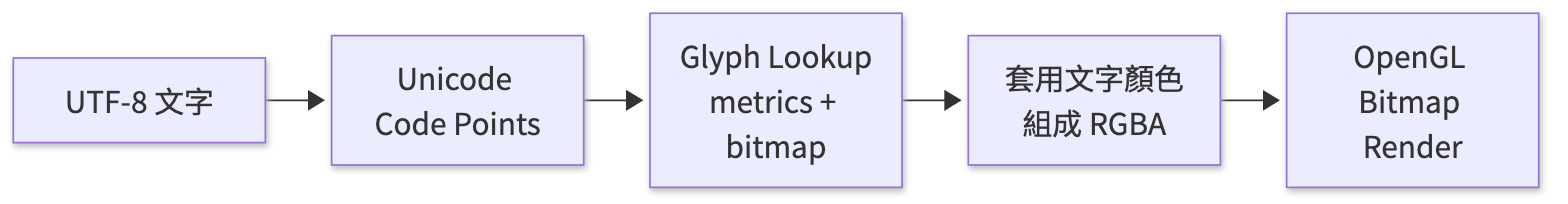
\includegraphics[width=.75\textwidth]{docs/figures/ch05_gfnt-runtime.png}
    \caption{UTF-8 字串到 GFNT 點陣字形的繪製流程}
    \label{fig:gfnt-runtime}
\end{figure}

\begin{figure}[htbp]
    \centering
    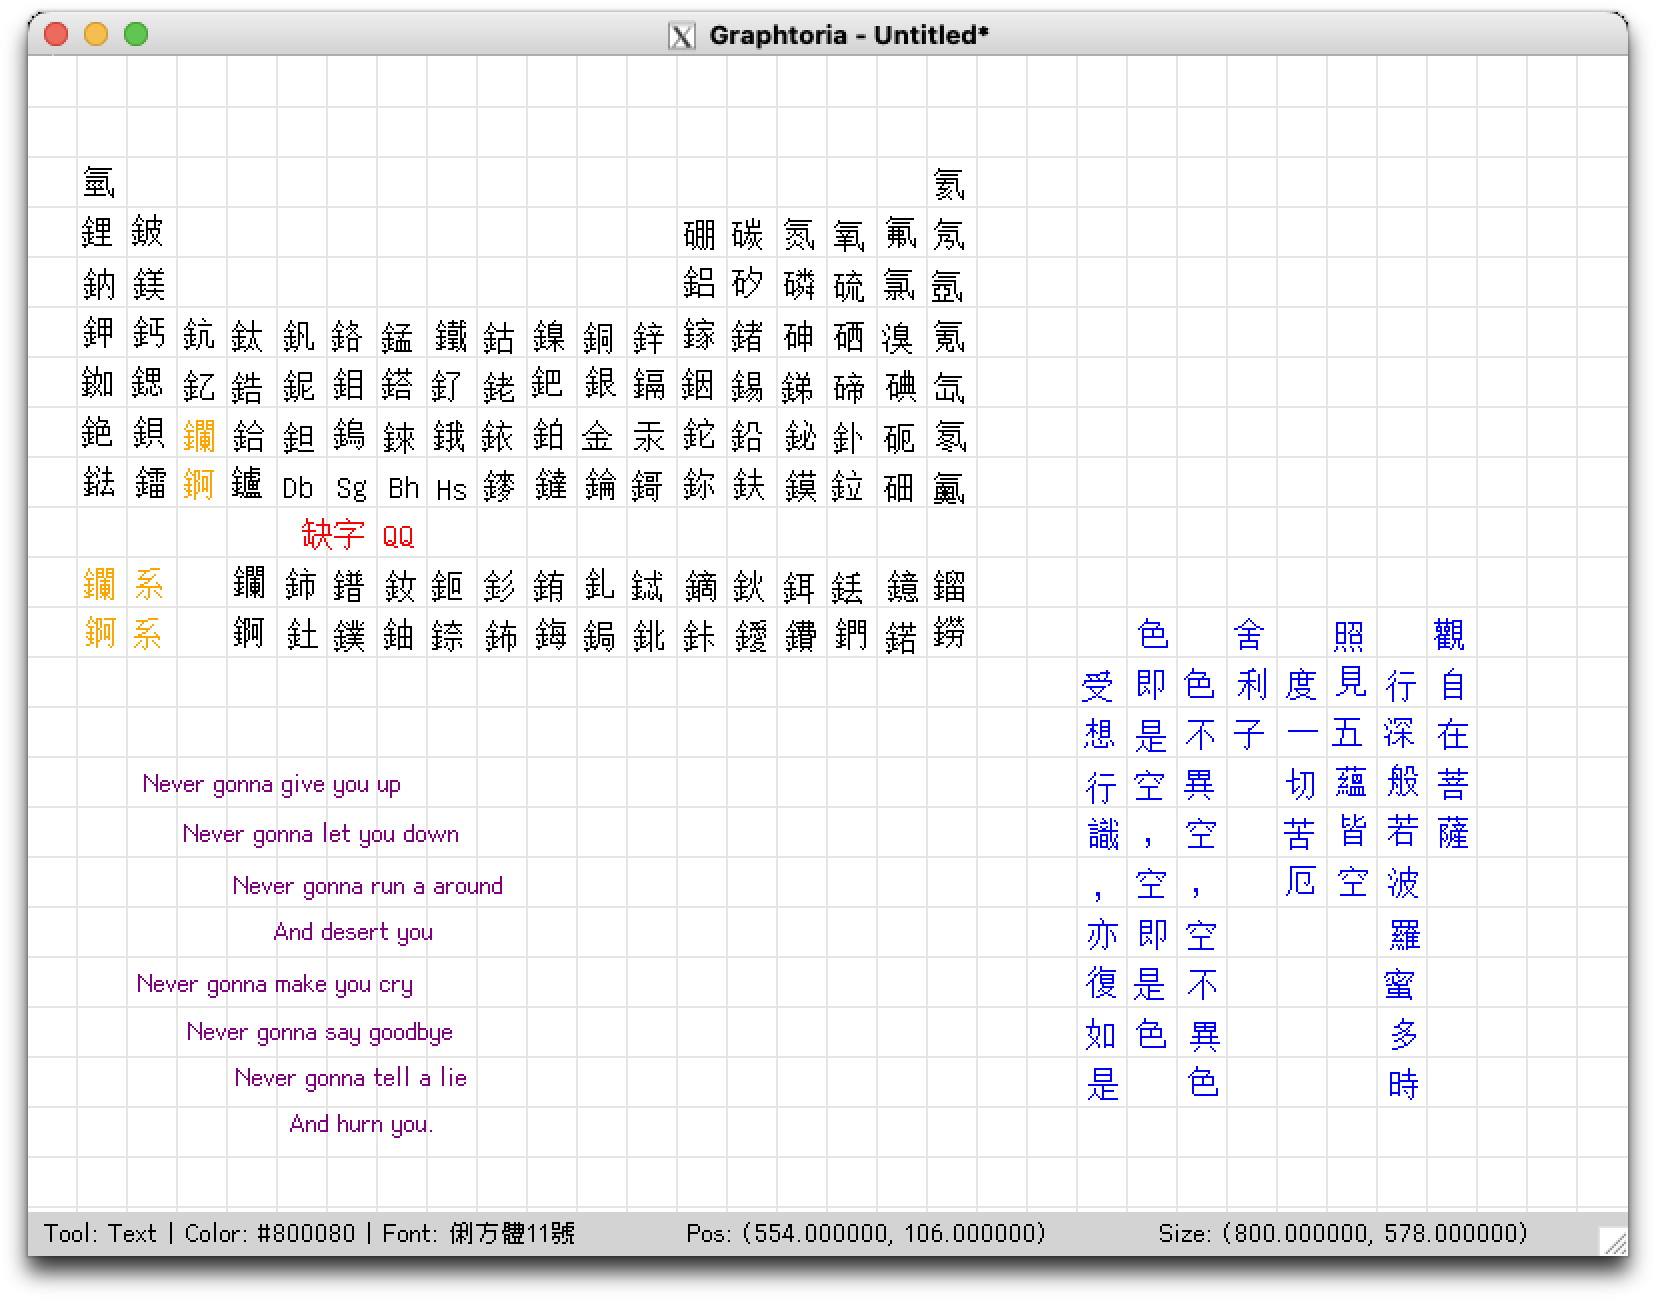
\includegraphics[width=.75\textwidth]{docs/figures/ch05_gfnt-chinese-output.png}
    \caption{GFNT 中文字型在 Graphtoria 中的實際輸出}
    \label{fig:gfnt-result}
\end{figure}
